\chapter{Hackystat-Trajectory - software process mining framework.}
the implementation of a system aiding in discovery of novel software process knowledge (shown at the Figure \ref{fig:system_overview});

\begin{figure}[tbp]
   \centering
   \includegraphics[height=65mm]{system_overview.eps}
   \caption{The high-level system overview. Software engineering process and product data collected and aggregated by Hackystat used to generate temporal symbolic indexes. Data mining tools constrained by the software engineering domain knowledge are then used for unsupervised patterns discovery. The GUI provides an expert interface for discovered patterns and knowledge base aiding iterative investigation of a discovered phenomena.}
   \label{fig:system_overview}
\end{figure}

\section{Framework overview.}

\section{Framework architecture.}

\section{Database schema design.}